\documentclass[10pt,portrait, twocolumn]{article}
\usepackage{multicol}
\usepackage{calc}
\usepackage[portrait]{geometry}
\usepackage{amsmath,amsthm,amsfonts,amssymb}
\usepackage{times}
\usepackage{color,graphicx,overpic}
\graphicspath{ {images/} }
\usepackage{hyperref}
\usepackage{pgfplots}
\usepackage{esint}
\usepackage{bm}
\usepackage{tikz}
\usepackage{relsize}
\usepackage{datetime}
\usepackage[utf8] {inputenc}
\usepackage[spanish, activeacute] {babel}
\usepackage{IEEEtrantools}
\usepackage{framed}

\usepackage{pdflscape}

\usepackage{draftwatermark}
\SetWatermarkText{Javier de Martín}
\SetWatermarkScale{0.8}

% This sets page margins to .5 inch if using letter paper, and to 1cm
% if using A4 paper. (This probably isn't strictly necessary.)
% If using another size paper, use default 1cm margins.
\geometry{top=.5cm,left=.5cm,right=.5cm,bottom=.5cm}
    
\pgfplotsset{
    dirac/.style={
        mark=triangle*,
        mark options={scale=2},
        ycomb,
        scatter,
        visualization depends on={y/abs(y)-1 \as \sign},
        scatter/@pre marker code/.code={\scope[rotate=90*\sign,yshift=-2pt]}
    }
}

% Turn off header and footer
\pagestyle{empty}

% Redefine section commands to use less space
\makeatletter
\renewcommand{\section}{\@startsection{section}{1}{0mm}%
                                {-1ex plus -.5ex minus -.2ex}%
                                {0.5ex plus .2ex}%x
                                {\normalfont\large\bfseries}}
\renewcommand{\subsection}{\@startsection{subsection}{2}{0mm}%
                                {-1explus -.5ex minus -.2ex}%
                                {0.5ex plus .2ex}%
                                {\normalfont\normalsize\bfseries}}
\renewcommand{\subsubsection}{\@startsection{subsubsection}{3}{0mm}%
                                {-1ex plus -.5ex minus -.2ex}%
                                {1ex plus .2ex}%
                                {\normalfont\small\bfseries}}
\makeatother

\newcommand{\Lagr}{\mathcal{L}}

% Define BibTeX command
\def\BibTeX{{\rm B\kern-.05em{\sc i\kern-.025em b}\kern-.08em
    T\kern-.1667em\lower.7ex\hbox{E}\kern-.125emX}}

% Don't print section numbers
\setcounter{secnumdepth}{0}


\setlength{\parindent}{0pt}
\setlength{\parskip}{0pt plus 0.5ex}

%My Environments
\newtheorem{example}[section]{Example}
% ---------------------------------------------------------------

\begin{document}


\begin{framed}
	\begin{center}
    	\Large{\underline{Redes de Transporte}} \\
    	\scriptsize{3º Ingeniería de Telecomunicaciones | UPV/EHU}\\
     	%Actualizado por última vez el \today \\
     	"\textsl{Under-promise and over-deliver}." \\
     	%\hspace{5 pt} \\
     	\small{\textbf{Javier de Martín -- 2016}}
	\end{center}
\end{framed}

%%%%%%%%%%%%%%%%%%%%%%%%%%%%%%%%%%%%%%%%%%%%%%%%%%%%%%%%%%%%%%%%%
% Tema 4

\section{\underline{0.- Introducción}}

Las redes de \textbf{acceso} hacen llegar la información del origen al primer equipo de red. Las redes de \textbf{transporte} llevan la información a través de la red, realiza las tareas de conmutación (nivel 2) y encaminamiento (nivel 3), transmisión y señalización.

\hrulefill

\section{\underline{1.- Encaminamiento}}

\textbf{Encaminar} consiste en establecer una ruta óptima para una instancia de comunicación desde una fuente a un destino. La ruta elegida debe optimizar en lo posible algún parámetro o conjunto de ellos. Las decisiones de encaminamiento son incrementales, cada nodo sólo debe decidir a qué nodo adyacente debe transmitir los datos.

\begin{itemize}
	\item \textbf{Algoritmo de encaminamiento}: Dado un destino decide la línea de salida adecuada.
	\item \textbf{Tabla de encaminamiento}: Estructura de información donde almacenar localmente los pares destino-salida.
	\item \textbf{Protocolo de encaminamiento}: Coordinación entre nodos del cálculo de las rutas e informar de entre sí de los cambios que se produzcan, por ejemplo, en la topología de la red.
\end{itemize}

Los encaminamientos deben de ser \textbf{robustos} para adaptarse a los posibles cambios de topología sin necesidad de abortar o reiniciar la red, \textbf{estables} en el sentido de converger a un resultado lo más rápido posible, no deben de generar \textbf{bucles} en el encaminamiento y no deben \textbf{favorecer} a ningún usuario frente a otro sin motivo.

\subsection{Encaminamiento IP}

En función de \textbf{dónde se decide encaminar}:

	\begin{itemize}
		\item \textbf{Fijado en el origen (Source Routing)}: Son los sistemas finales los que fijan la ruta que ha de seguir cada paquete. Cada paquete lleva un campo que especifica su ruta (RI, Routing Information), y los nodos sólo se dedican a reenviar los paquetes por esas rutas ya especificadas. Los sistemas finales son los que tienen las tablas de encaminamiento y no se hace necesaria la consulta o existencia de tablas de encaminamiento en los nodos intermedios. El nodo origen debe de conocer la topología de la red. No existen bucles, el sistema final fija la ruta.
		\item \textbf{Salto a Salto (Hop by Hop)}: Los nodos, en función del destino, conocen sólo el siguiente salto a realizar. Pueden ocurrir bucles, no se tiene una visión completa de la red.
	\end{itemize}
	
En función de la \textbf{adaptabilidad}:

	\begin{itemize}
		\item \textbf{No adaptables (estáticos)}:
			\begin{itemize}
				\item Estáticos: Las tablas de encaminamiento de los nodos se configuran de forma manual y permanecen inalterables hasta que no se vuelve a actuar sobre ellas. Tanto la recogida como la distribución de información se realiza por gestión (manera externa a la red), sin ocupar capacidad de red. Es óptimo para topologías de red en las que sólo hay una posibilidad de encaminamiento (topología en estrella).
				\item Q-Estáticos: Igual que el estático pero en vez de dar una sola ruta fija se proporcionan varias alternativas en caso de que la principal no funcione. Tiene adaptabilidad reducida.
			\end{itemize}
		\item \textbf{Adaptables (dinámicos)}:
			\begin{itemize}
				\item Centralizados: Los nodos envían a un nodo central la información de control acerca de sus vecinos. El nodo central será el que se encargue de recoger esta información de control acerca de sus vecinos. El nodo central será el que se encargue de recoger esta información para construir la tabla de encaminamiento de cada nodo en función de la información de control que éstos le mandan. Tiene un alto consumo de recursos de la red y se necesita disponer de rutas alternativas (y nodo central alternativo) para comunicarse con el nodo central, ya que estos métodos dejarían de funcionar con la caída de éste.
				\item Aislados: El más simple, no tiene en cuenta la información de los otros nodos a la hora de encaminar. Cada vez que un nodo recibe un paquete que tiene que reenviar (porque no es para él) lo reenvía por todos los enlaces salvo por el que le llegó (inundación). Útil para enviar información de emergencia ya que se asegura que llega a todos los nodos.
				\item Distribuidos: Todos los nodos son iguales, todos envían y reciben información de control y todos calculan, a partir de su RIB (base de información de encaminamiento) sus tablas de encaminamiento. La adaptación a cambios es óptima siempre y cuando éstos sean notificados.
			\end{itemize}
	\end{itemize}

\begin{center}
\begin{tabular}{|l|l|l|l|}
\hline
\textbf{Encaminamiento} & \textbf{Info de Control} & \textbf{Decisión} & \textbf{Adaptación} \\ \hline
\textbf{Estáticos}               & No                              & Offline                             & No                                \\ \hline
\textbf{Cuasiestáticos}          & No                              & Offline                             & Reducida                          \\ \hline
\textbf{Centralizado}            & Nodo Central                    & Nodo Central                        & Si                                \\ \hline
\textbf{Distribuido}             & Entre Nodos                     & Cada Nodo                           & Si                                \\ \hline
\textbf{Aislado}                 & no                              & Cada Nodo                           & Si                                \\ \hline
\end{tabular}
\end{center}

En el encaminamiento \textbf{estático} la tabla de encaminamiento de los equipos se actualiza de forma manual y en el \textbf{dinámico} se actualiza mediante protocolos de encaminamiento.

\subsection{Encaminadores o Routers}

Un \textbf{router} tiene que encontrar una ruta y encaminar los datos. \textit{Routing} es el proceso de decidir a dónde enviar un paquete recibido utilizando la tabla de encaminamiento del router y \textit{forwarding} es el acto de enviar el paquete al siguiente salto.\\

Los routers tienen dos tablas clave:

	\begin{itemize}
		\item \textbf{FIB} (Forwarding table): Contiene destinos y las interfaces para llegar a ellos. El router la utilizar para descubrir la interfaz a la que enviar los paquetes. A veces se confunden con rutas (\textbf{no entiendo esto}).
		\item \textbf{RIB} (Routing table): Contiene una lista de los destinos alcanzables y los siguientes saltos para alcanzar los destinos. Un destino puede ser alcanzado a través de varios posibles next hops pero sólo el mejor va a la FIB.
	\end{itemize}
	
	\begin{center}
		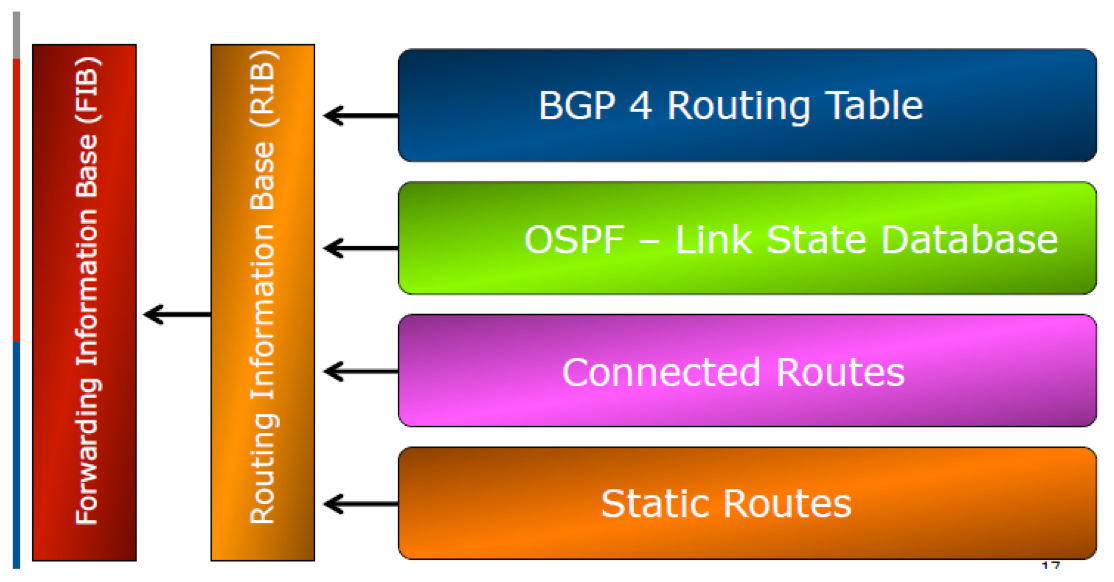
\includegraphics[scale = .5]{FIBRIB}
	\end{center}
	
\subsection{Encaminamiento IP}

El protocolo IP es un protocolo \textbf{no fiable} (best effort), \textbf{no orientado a conexión}, no mantiene \textbf{información de estado}, los datagramas pueden llegar fuera de secuencia con errores o pérdidas, es el protocolo de nivel superior el encargado de resolver estos problemas. \\

IP realiza tiene dos tipos de encaminamiento:

	\begin{itemize}
		\item \textbf{Directo}: Un equipo puede enviar un paquete IP a otra máquina sin pasar por un tercer equipo. En la misma red.
		\item \textbf{Indirecto}: Un equipo quiere enviar un paquete IP a otro equipo y tiene que atravesar una ruta de otros equipos. En distintas redes.
	\end{itemize}

La tabla de encaminamiento IP en cada equipo incluye un conjunto de direcciones IP destino y las direcciones IP del siguiente salto para cada destino. Además, pueden incluir para llegar a destinos rutas directas, indirectas o por defecto. \\

El algoritmo de encaminamiento IP es el siguiente:
	\begin{center}
		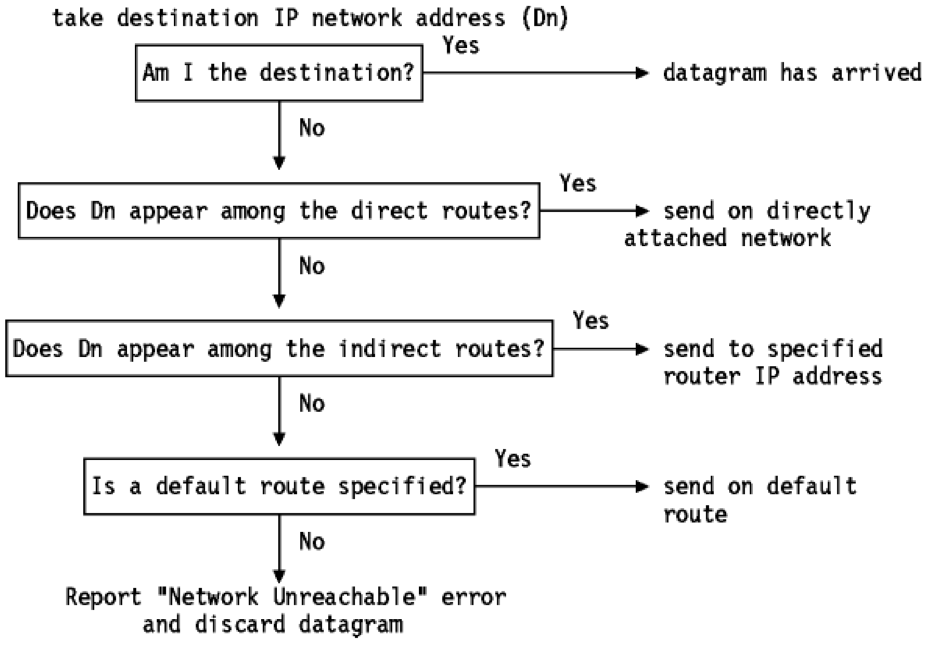
\includegraphics[scale = .5]{AlgoritmoIP}
	\end{center}


\hrulefill
	
	
	
%\vfill




%\end{multicols}

\end{document}